\documentclass{entcs} 
\usepackage{entcsmacro}

\usepackage{fancyvrb}
\usepackage{listings}
% Packages.tex

% Packages di latex utilizzati 

  % Standard dell'ams
\usepackage{amssymb,amsmath}

  % Per le definizioni di connessioni di Galois
\usepackage{galois}

  % Per formattare ed includere il testo
\usepackage{lgrind}
     % Cambiamento dei font per lgrind: tutti in Courier
\def\CMfont{\ttfamily\itshape}
\def\KWfont{\ttfamily\bfseries}
\def\VRfont{\ttfamily}
\def\BGfont{\ttfamily}
\def\NOfont{\ttfamily}

  % Caratteri speciali per i nomi di funzione
\usepackage{bbm}

  % Caratteri ``cal'' carini
\usepackage[mathcal]{euscript}

  % per \baro
\usepackage{stmaryrd}

  % per \xspace
\usepackage{xspace}

  % per i diagrammi
\usepackage[all]{xy}

  % for scalebox
\usepackage{graphicx}
 
   % Per le figure incastrate l'una nell'altra
\usepackage{subfigure}

  % Per le figure nel testo
\usepackage{wrapfig}

\usepackage{listings}

\usepackage{tabularx}

  % Per includere i verbatim
\newbox\subfigbox
\makeatletter
\newenvironment{subfloat}
{\def\caption##1{\gdef\subcapsave{\relax##1}}%
\let\subcapsave\@empty
\setbox\subfigbox\hbox
\bgroup}
{\egroup
\subfigure[\subcapsave]{\box\subfigbox}}
\makeatother

   % Per la compilazione Condizionale
\usepackage{ifthen}

   % Per i riferimenti incrociati

%\ifx\pdfoutput\undefined % Se compilo con ``latex'' ed uso ps2pdf
%\usepackage{color}
%\usepackage[dvips]{graphicx}       %%% graphics for dvips
%\DeclareGraphicsExtensions{.eps}   %%% standard extension for included graphics
%\usepackage[bookmarks=true]{hyperref}
%\else                    % Se compilo con ``pdflatex'' 
%\usepackage[pdftex]{graphicx}      %%% graphics for pdfLaTeX 
%\DeclareGraphicsExtensions{.pdf}   %%% standard extension for included graphics
%\usepackage[pdftex]{thumbpdf}      %%% thumbnails for pdflatex
%\usepackage[pdftex,                %%% hyper-references for pdflatex
%bookmarks=true,%                   %%% generate bookmarks ...
%bookmarksnumbered=true,%           %%% ... with numbers
%hypertexnames=false,%              %%% needed for correct links to figures !!!
%breaklinks=true,%                  %%% break links if exceeding a single line
%linkbordercolor={0 0 1}]{hyperref} %%% blue frames around links
%                                  %%% pdfborder={0 0 1} is the default
%\hypersetup{
%pdfauthor   = {Francesco Logozzo \& Agostino Cortesi},
%pdftitle    = {to be decided},
%pdfsubject  = {Objects},
%pdfkeywords = {Abstract Interpretation, Static Analysis, Object Oriented}
%}
%\pdfadjustspacing=1                %%% force LaTeX-like character spacing
%\fi 


%%% Local Variables: 
%%% mode: plain-tex
%%% TeX-master: "main"
%%% End: 

% Definizione dei simboli

\newcommand{\eg}{\textit{e.g.}}
\newcommand{\ie}{\textit{i.e.}}

% Definizione dell' operatore di astrazione
\newcommand{\abs}[1]{\ensuremath{\bar{\mathsf{#1}}}}

\newcommand{\sx}{\llbracket}
\newcommand{\dx}{\rrbracket}

  % Semantica generica
\newcommand{\sem}[1]{\ensuremath{\sx \mathtt{#1} \dx}}

  % Semantica che prende un nome
\newcommand{\semantica}[2]{\ensuremath{\mathbb{#1}\sem{#2}}}

\newcommand{\BigSemantica}[2]{\ensuremath{\mathbb{#1}{\Bigg\llbracket #2 \Bigg\rrbracket}}}

  % Semantiche generiche
\newcommand{\csem}[1]{\ensuremath{\semantica{s}{#1}}}
\newcommand{\asem}[1]{\ensuremath{\semantica{\abs{s}}{#1}}}
\newcommand{\asemRefined}[1]{\ensuremath{\semantica{\abs{s}^*}{#1}}}

  % Funzione di ``transfer''
\newcommand{\trasf}[1]{\ensuremath{\semantica{t}{#1}}}
\newcommand{\atrasf}[1]{\ensuremath{\semantica{\abs{t}}{#1}}}

  % Semantica di: costruttore,  metodo
\newcommand{\semcostr}[1]{\semantica{i}{#1}}
\newcommand{\semmetodo}[1]{\semantica{m}{#1}}
\newcommand{\semoggetto}[1]{\semantica{o}{#1}}
\newcommand{\semclasse}[1]{\semantica{c}{#1}}

  % Semantica Colleting Traces
\newcommand{\Semmetodo}[1]{\semantica{M}{#1}}
\newcommand{\Semoggetto}[1]{\semantica{O}{#1}}
\newcommand{\Semclasse}[1]{\semantica{C}{#1}}

  % Semantics Reachable States
\newcommand{\rsemcostr}[1]{\semantica{I}{#1}}
\newcommand{\rsemmetodo}[1]{\Semmetodo{#1}}
\newcommand{\rsemoggetto}[1]{\semantica{O}{#1}}
\newcommand{\rsemclasse}[1]{\semantica{C}{#1}}

  % Seamntica Astratta
\newcommand{\asemcostr}[1]{\semantica{\bar{I}}{#1}}
\newcommand{\asemmetodo}[1]{\semantica{\bar{M}}{#1}}
\newcommand{\asemoggetto}[1]{\semantica{\bar{O}}{#1}}
\newcommand{\asemclasse}[1]{\semantica{\bar{C}}{#1}}

  % Operazioni su stati
\newcommand{\less}{\ensuremath{\sqsubseteq}}
\newcommand{\join}{\ensuremath{\sqcup}}
\newcommand{\meet}{\ensuremath{\sqcap}}
\newcommand{\bottom}{\ensuremath{\bot}}
\newcommand{\bigjoin}{\ensuremath{\bigsqcup}}

  % Semantica astratta
\newcommand{\asemantica}[2]{\semantica{\bar{#1}}{#2}}
\newcommand{\asemanticaBig}[2]{\BigSemantica{\bar{#1}}{#2}}


  % Semantica astratta BIS, per aggiungere pedici
\newcommand{\asemanticaBis}[3]{\semantica{\bar{#1}_{\textit{#2}}}{#3}}

  % Operazioni astratte
\newcommand{\nabs}[1]{\bar{#1}}
\newcommand{\abot}{\nabs{\bot}}
\newcommand{\atp}{\nabs{\ensuremath{\top}}}
\newcommand{\aless}{\nabs{\less}}
\newcommand{\asup}{\ensuremath{\nabs{\sqsupseteq}}}
\newcommand{\acup}{\ensuremath{\nabs{\sqcup}}}
\newcommand{\ajoin}{\acup}
\newcommand{\abigcup}[1]{\nabs{\bigsqcup_{#1}}}
\newcommand{\abigjoin}[1]{\abigcup{#1}}
\newcommand{\acap}{\ensuremath{\nabs{\sqcap}}}
\newcommand{\ameet}{\acap}
\newcommand{\abigcap}[1]{\nabs{\bigsqcap_{#1}}}
\newcommand{\abigmeet}[1]{\abigcap{#1}}


 % lfp : least fixpoint
\newcommand{\lfp}[2]{\ensuremath{\mathrm{lfp}^{#1}_{#2}}}

 % gfp: greatest fixpoint
\newcommand{\gfp}[2]{\ensuremath{\mathrm{gfp}^{#1}_{#2}}}


% Insiemi e Funzioni

  % Insieme, elemento di insieme, nessun elemento
\newcommand{\insieme}[1]{\ensuremath{\mathsf{#1}}}
\newcommand{\el}[1]{\ensuremath{\mathsf{#1}}}
\newcommand{\noel}{\el{\bot}}

  % Insieme delle parti
\newcommand{\parti}[1]{\ensuremath{\mathcal{P}{(#1)}}}
\newcommand{\partiFin}[1]{\ensuremath{\mathcal{P}_{\mathrm{fin}}{(#1)}}}


  % Elementi di insiemi
\newcommand{\noval}{\ensuremath{\baro}}

  % Cardinalita di inisiemi
\newcommand{\cardinalita}[1]{\ensuremath{\# #1}}

  % Env, Store, Addr, Val, Label : Scorciatoie
\newcommand{\env}{\insieme{Env}}
\newcommand{\Env}{\env}

\newcommand{\aenv}{\ensuremath{\bar{\env}}}

\newcommand{\store}{\insieme{Store}}
\newcommand{\Store}{\store}

\newcommand{\astore}{\ensuremath{\overline{\store}}}

\newcommand{\AState}{\abs{\Sigma}}
\newcommand{\astate}{\AState}

\newcommand{\addr}{\insieme{Addr}}
\newcommand{\Addr}{\addr}

\newcommand{\aaddr}{\ensuremath{\overline{\addr}}}

\newcommand{\Reference}{\insieme{Ref}}
\newcommand{\reference}{\reference}

\newcommand{\AReference}{\ensuremath{\overline{\Reference}}}

\newcommand{\val}{\insieme{Val}}

\newcommand{\etichetta}{\insieme{Label}}
\newcommand{\cont}{\ensuremath{\kappa}}

  % Stati
\newcommand{\stati}[1]{\ensuremath{\Sigma}}
  % Tracce
\newcommand{\tracce}[1]{\ensuremath{\mathcal{T}(#1)}}
  % Transizione
\newcommand{\tr}[1]{\ensuremath{\xrightarrow{#1}}}

  % Insieme di funzioni
\newcommand{\funzione}[2]{\ensuremath{[#1 \rightarrow#2]}}

  % Funzione vuota
\newcommand{\emptyfun}{\ensuremath{[\cdot]}}

  % Insieme di funzioni monotone e joim-morphism
\newcommand{\funmon}[2]{\ensuremath{[#1 \stackrel{m}{\longrightarrow} #2]}}
\newcommand{\funjoin}[2]{\ensuremath{[#1 \stackrel{\sqcap}{\longrightarrow} #2]}}

% Astratto
  % Dominio concreto
\newcommand{\dom}[1]{\insieme{#1}}

  % Dominio astratto
\newcommand{\adom}[1]{\ensuremath{{\mathsf{#1}}}}

 % Vari domini
\newcommand{\Intervals}{\dom{Intv}}
\newcommand{\LT}{\dom{LT}}
\newcommand{\Boxes}{\dom{Boxes}}
\newcommand{\DBM}{\dom{DBM}}
\newcommand{\Octagons}{\dom{Oct}}
\newcommand{\Polyhedra}{\dom{Poly}}
\newcommand{\Poly}{\Polyhedra}
\newcommand{\Lineq}{\dom{LinEq}}
\newcommand{\LinEq}{\Lineq}
\newcommand{\Karr}{\Lineq}
\newcommand{\Symbolic}{\dom{Symb}}
\newcommand{\Pentagons}{\dom{Pnt}}
\newcommand{\SubPolyhedra}{\dom{SubPoly}}
\newcommand{\SubPoly}{\SubPolyhedra}
\newcommand{\Subpoly}{\SubPolyhedra}

  % Elemento di dominio astratto
\newcommand{\ael}[1]{\ensuremath{\abs{\el{#1}}}}
\newcommand{\aelBis}[2]{\ensuremath{\abs{\el{#1}}_\el{#2}}}

  % Funzione di astrazione e concretizzazione
\newcommand{\alfa}{\ensuremath{\alpha}}
%\renewcommand{\gamma}{\ensuremath{\gamma}}
\newcommand{\gm}{\ensuremath{\gamma}}


% Funzioni usate nella tesi
  % Transizione basica
\newcommand{\prossimo}{\ensuremath{\mathrm{next}}}
%\newcommand{\next}{\ensuremath{\mathrm{next}}}
\newcommand{\nextDir}{\ensuremath{\mathrm{next_{dir}}}}
\newcommand{\nextInd}{\ensuremath{\mathrm{next_{ind}}}}
\newcommand{\prossimoDir}{\nextDir}
\newcommand{\prossimoInd}{\nextInd}

  % Transizione ``collecting''
\newcommand{\Next}{\ensuremath{\mathrm{Next}}}
\newcommand{\NextDir}{\ensuremath{\mathrm{Next_{dir}}}}
\newcommand{\NextInd}{\ensuremath{\mathrm{Next_{ind}}}}

  % Reachable addresses
\newcommand{\reachable}{\ensuremath{\mathrm{reachable}}}
  % Update function
\newcommand{\update}{\ensuremath{\mathrm{update}}}
  % Storia delle interazioni
%\newcommand{\etichette}{\ensuremath{\mathrm{labels}}}
\newcommand{\storia}{\ensuremath{\mathrm{history}}}

  % Contesto
\newcommand{\contesto}{\ensuremath{\mathrm{Context}}}

  % Contesto Astratto
\newcommand{\acontesto}{\ensuremath{\mathrm{\overline{Context}}}}

% Tracce : definizioni
\newcommand{\stringavuota}{\ensuremath{\epsilon}}


% Funzioni di astrazione
  % Prima Astrazione, quella dei metodi
\newcommand{\alfaPrima}{\ensuremath{\alpha_{\Yright}}}
\newcommand{\gammaPrima}{\ensuremath{\gamma_{\Yright}}}
  % Versione higher-order
\newcommand{\alfaPrimaDot}{\ensuremath{\dot{\alpha}_{\Yright}}}

  % Seconda Astrazione, quella degli stati
\newcommand{\alfaSeconda}{\ensuremath{\alpha_{\circ}}}
\newcommand{\gammaSeconda}{\ensuremath{\gamma_{\circ}}}
  % Versione higher-order
\newcommand{\alfaSecondaDot}{\ensuremath{\dot{\alpha}_{\circ}}}


\newcommand{\alfaAddr}{\ensuremath{\alpha_\el{a}}}
\newcommand{\gammaAddr}{\ensuremath{\gamma_\el{a}}}

\newcommand{\gammaBool}{\ensuremath{\gamma_\el{b}}}

\newcommand{\gammaEnv}{\ensuremath{\gamma_\el{e}}}

\newcommand{\gammaOct}{\ensuremath{\gamma_\el{o}}}
\newcommand{\gammaDOct}{\ensuremath{\gamma_\el{do}}}

\newcommand{\gammaRef}{\ensuremath{\gamma_\el{r}}}

\newcommand{\gammaStore}{\ensuremath{\gamma_\el{s}}}

\newcommand{\gammaState}{\ensuremath{\gamma_{\astate}}}

% Estensioni per OO

  % Classe
\newcommand{\classe}[1]{\ensuremath{\mathtt{#1}}}
\newcommand{\classi}{\ensuremath{\mathcal{C}}}

  % Gerarchia
\newcommand{\gerarchia}[1]{\ensuremath{\mathcal{#1}}}
\newcommand{\gerarchie}{\ensuremath{\mathbb{H}}}

  % Operatori su Gerarchie 
\newcommand{\inserisciClasse}{\ensuremath{\uplus}}
\newcommand{\costruisciClasse}{\ensuremath{\beta}}
\newcommand{\unisciGerarchie}{\ensuremath{\Cup}}

\newcommand{\aclasse}[1]{\ensuremath{\abs{\mathtt{#1}}}}
\newcommand{\aclasseLong}[1]{\ensuremath{\overline{\mathtt{#1}}}}
  % Oggetto, instanza di classe
\newcommand{\oggetto}[1]{\ensuremath{\mathsf{#1}}}
  % Metodo
\newcommand{\metodo}[1]{\ensuremath{\mathtt{#1}}}
  % Campo
\newcommand{\campo}[1]{\ensuremath{\mathtt{#1}}}

  % Astrazioni di campi
\newcommand{\acampo}[1]{\ensuremath{\mathtt{\abs{#1}}}}

  % Astrazione di metodi con constraints
\newcommand{\ametodo}[1]{\ensuremath{\mathtt{\abs{#1}}}}

% Dominio delle Tracce Collecting

\newcommand{\adomTracce}{\ensuremath{\adom{D}_{\Yright}}}

\newcommand{\atopTracce}{\ensuremath{\abs{\top}_{\Yright}}}
\newcommand{\abottomTracce}{\ensuremath{\abs{\bot}_{\Yright}}}

\newcommand{\alessTracce}{\ensuremath{\abs{\subseteq}_{\Yright}}}
\newcommand{\alessTraccia}{\ensuremath{\abs{\subseteq}^{\tau}_{\Yright}}}

\newcommand{\ajoinTracce}{\ensuremath{\abs{\cup}_{\Yright}}}
\newcommand{\ajoinTraccia}{\ensuremath{\abs{\cup}^{\tau}_{\Yright}}}

\newcommand{\ameetTracce}{\ensuremath{\abs{\cap}_{\Yright}}}
\newcommand{\ameetTraccia}{\ensuremath{\abs{\cap}^{\tau}_{\Yright}}}

% Scorciatoie

  % ``Prende''
\newcommand{\prende}{\ensuremath{\mapsto}}

  % Simbolo di definizione
\newcommand{\df}{\ensuremath{\triangleq}}

  % Tupla
\newcommand{\tupla}[1]{\ensuremath{\langle #1 \rangle}}

  % Stati Iniziali
\newcommand{\statiiniziali}[1]{\ensuremath{S_0\tupla{#1}}}

  % Modularita
\newcommand{\hasA}{has-A}
\newcommand{\isA}{is-A}

  % Riferimento ad una formula
\newcommand{\formula}[1]{\ensuremath{\mathrm{(\ref{#1})}}}

% Complessita

  % O-notation
\newcommand{\costo}[1]{\ensuremath{\kappa_{#1}}}


% Definizioni per i domini di vincoli

\newcommand{\Vars}{\ensuremath{\mathtt{Vars}}}
\newcommand{\C}{\ensuremath{\dom{C}}}
\newcommand{\initC}{\ensuremath{\mathrm{initial_{\C}}}}

\newcommand{\dominio}{\ensuremath{\mathrm{dom}}}
\newcommand{\range}{\ensuremath{\mathrm{range}}}

  % Relazioni
\newcommand{\rel}[1]{\ensuremath{\mathsf{\rho}[\mathtt{#1}]}}
\newcommand{\conDuepar}[2]{\ensuremath{\con'[\mathtt{#1}, \mathtt{#2}]}}
\newcommand{\conTrepar}[3]{\ensuremath{\con[\mathtt{#1}, \allowbreak \mathtt{#2}, \allowbreak \mathtt{#3}]}}
\newcommand{\relass}[1]{\ensuremath{\rho(#1)}}

\newcommand{\rgamma}{\ensuremath{\gamma_{\rho}}}
\newcommand{\cgamma}{\ensuremath{\gamma_{\C}}}

 % Lettera
\newcommand{\con}{\ensuremath{\mathsf{c}}}

 % Sequenza
\newcommand{\seq}[1]{\ensuremath{\vartriangleright_\mathtt{#1}}}


 % Semantiche per i vincoli
\newcommand{\semc}[1]{\semantica{s}{#1}}

\newcommand{\semtracce}[1]{\semantica{t}{#1}}
\newcommand{\asemtracce}[1]{\semantica{\bar{t}}{#1}}
\newcommand{\asemtracces}[1]{\semantica{\bar{s}}{#1}}


\newcommand{\modsem}[1]{\ensuremath{\semantica{T}{#1}}}
\newcommand{\amodsem}[1]{\semantica{\bar{T}}{#1}}

\newcommand{\A}{\ensuremath{\adom{A}}\xspace}
\newcommand{\modA}{\ensuremath{\adom{A}_\mathsf{M}}\xspace}
\newcommand{\Absel}{\ensuremath{\ael{a}}\xspace}
\newcommand{\modAbsel}{\ensuremath{\ael{a}_\mathsf{m}}\xspace}

\newcommand{\relsem}[1]{\semantica{R}{#1}}

 % Proiezione/dropping

\newcommand{\lascia}{\ensuremath{\delta}}
\newcommand{\tieni}{\ensuremath{\pi}}

%\newcommand{\Absless}{\ensuremath{\sqsubseteq^\mathsf{a}}}
\newcommand{\modAbsless}{\ensuremath{\abs{\sqsubseteq}_\mathsf{m}}}

%\newcommand{\Absjoin}{\ensuremath{\sqcap^\mathsf{a}}}
\newcommand{\modAbsjoin}{\ensuremath{\abs{\sqcap}_\mathsf{m}}}

\newcommand{\aconc}{\ensuremath{\abs{\odot}}\xspace}


 % Operazioni sul dominio di vincoli
\newcommand{\cless}{\ensuremath{\preceq}}
\newcommand{\cgreater}{\ensuremath{\succeq}}
\newcommand{\ctop}{\ensuremath{\vernal}}
\newcommand{\cbot}{\ensuremath{\bot^\con}}
\newcommand{\cmeet}{\ensuremath{\curlywedge}}
\newcommand{\cjoin}{\ensuremath{\curlyvee}}
\newcommand{\cwiden}{\ensuremath{\hbox{\hbox to 0pt{\raisebox{4pt}{$\relbar$}}$\curlyvee$}}}
\newcommand{\bigcjoin}{\ensuremath{\bigcurlyvee}}

\newcommand{\alg}{\ensuremath{\mathcal{A}}}

 % Definizione di BodyOf
\newcommand{\bodyof}[1]{\ensuremath{\mathrm{bodyOf}(\mathbf{#1})}}

 % Definitione di tiedVars
\newcommand{\tiedvars}{\ensuremath{\mathrm{tiedVars}}}

  % Operazioni su Tracce
%\newcommand{\tracce}[1]{\ensuremath{\wp(#1^\infty)}\xspace}
\newcommand{\iniziatracce}[2]{\ensuremath{\mathcal{T}(#1,#2)}}
\newcommand{\giunzione}{\ensuremath{\frown}\xspace}
\newcommand{\conc}{\ensuremath{\odot}\xspace}
\newcommand{\last}{\ensuremath{\mathrm{last}}}

  % Funzioni Semantiche ``Astratte''
\newcommand{\flow}[1]{\ensuremath{\mathrm{flow}_\mathtt{#1}}}
\newcommand{\aflow}[1]{\ensuremath{\overline{\mathrm{flow}}_\mathtt{#1}}}

  % Definizione di ``approssima'', i.e. un vincolo approssima la semantica di un metodo
\newcommand{\approssima}{\ensuremath{\Subset}}

  % Approssimazione con vincoli della semantica di un metodo
\newcommand{\conmetodo}[5]{\ensuremath{\con_{#1}[\mathtt{#2}, \allowbreak \mathtt{#3}, \allowbreak \mathtt{#4}, \allowbreak \mathtt{#5}]}}



% Definizione del dominio degli osservabili
\newcommand{\osservabile}[2]{\ensuremath{\mathcal{O}_{#2}(\classe{#1})}}
\newcommand{\oless}{\ensuremath{{\sqsubseteq}_{o}}}
\newcommand{\osup}{\ensuremath{{\sqsupseteq}_{o}}}
\newcommand{\ojoin}{\ensuremath{{\sqcup}_{o}}}
\newcommand{\omeet}{\ensuremath{{\sqcap}_{o}}}
\newcommand{\otp}{\ensuremath{{\top}_{o}}}
\newcommand{\obot}{\ensuremath{{\bot}_{o}}}
\newcommand{\obigjoin}{{{\bigsqcup}{}}_{o}}

\newcommand{\domPiuPreciso}{\ensuremath{O[\parti{\Sigma}]}}

% Interfaccia di una classe
\newcommand{\interfaccia}[1]{\ensuremath{\iota(\classe{#1})}}


% Definizione dell' insieme delle astrazioni di un dominio +
% operazioni

\newcommand{\astrazioni}[1]{\ensuremath{\mathcal{A}(#1)}}
\newcommand{\dless}{\ensuremath{\leq}}
\newcommand{\djoin}{\ensuremath{\vee}}
\newcommand{\dmeet}{\ensuremath{\wedge}}

% Dominio dei valori
\newcommand{\dominioVal}[1]{\ensuremath{\mathit{#1}}}

% Stato interno ad un oggetto
\newcommand{\stato}{\ensuremath{\sigma}}

% Semantica backward concreta ed astratta
\newcommand{\backSemmetodo}[1]{\semantica{{M}^{<}}{#1}}
\newcommand{\abacksemmetodo}[1]{\semantica{\bar{M}^{<}}{#1}}


% Complexity
\newcommand{\Order}[1]{\ensuremath{\mathcal{O}(#1)}}

% Keywords

\newcommand{\Clousot}{\ensuremath{\mathtt{Clousot}}}

\newcommand{\code}[1]{\ensuremath{\mathtt{#1}}}

\newcommand{\takes}{\ensuremath{\leftarrow}}

\newcommand{\linea}[1]{\ensuremath{#1}}



% Syntax

\newcommand{\Assert}{\ensuremath{\mathtt{assert}}~}
\newcommand{\Assume}{\ensuremath{\mathtt{assume}}~}
\newcommand{\While}{\code{while}}
\newcommand{\If}{\code{if}}
\newcommand{\Else}{\code{else}}
\newcommand{\Skip}{\code{skip}}

\newcommand{\Stm}{\code{Stm}}
\newcommand{\Var}{\code{Var}}
\newcommand{\Exp}{\code{Exp}}
\newcommand{\BExp}{\code{BExp}}
\newcommand{\Bexp}{\BExp}
\newcommand{\ExpTwoOps}{\code{ExpTwoOps}}
\newcommand{\Lit}{\code{Lit}}
\newcommand{\Op}{\code{op}}
\newcommand{\Relop}{\code{relop}}
\newcommand{\Int}{\code{int}}

\newcommand{\Code}{\code{IstrStream}}
\newcommand{\Label}{\code{Label}}
\newcommand{\Istr}{\code{Istr}}
\newcommand{\Jump}{\code{jmp}}
\newcommand{\JumpIfTrue}{\code{jmpIf}}
\newcommand{\JumpIf}{\JumpIfTrue}
\newcommand{\Nop}{\code{nop}}

\newcommand{\Comp}{\ensuremath{\mathcal{C}}}
\newcommand{\Compexp}{\ensuremath{\mathcal{C}_{e}}}
\newcommand{\CompExp}{\Compexp}

\newcommand{\assign}{\el{assign}}
\newcommand{\test}{\el{test}}
\newcommand{\guard}{\test}
\newcommand{\checkif}{\el{check}}
\newcommand{\checkIf}{\checkif}

\newcommand{\aassign}{\el{\assign}}
\newcommand{\atest}{\el{\test}}

\newcommand{\arange}{\el{\mathsf{range}}}

\newcommand{\widening}{\ensuremath{\triangledown}}
\newcommand{\awidening}{\widening}
\newcommand{\narrowing}{\ensuremath{\vartriangle}}

\newcommand{\HLsem}[1]{\asemantica{H}{#1}}
\newcommand{\HLSem}[1]{\HLsem{#1}}
\newcommand{\LLsem}[1]{\asemantica{L}{#1}}
\newcommand{\LLSem}[1]{\LLsem{#1}}

\newcommand{\BigLLSem}[1]{\asemanticaBig{L}{#1}}
\newcommand{\bigLLSem}[1]{\BigLLSem{#1}}
\newcommand{\bigLLsem}[1]{\BigLLSem{#1}}

\newcommand{\result}{\code{res}}

% Definizioni per Subpolyhedra


\newcommand{\VarProg}{\ensuremath{\Var_\mathtt{P}}}
\newcommand{\VarSlack}{\ensuremath{\Var_\mathtt{S}}}

\newcommand{\variable}[1]{\ensuremath{\mathtt{#1}}}

\newcommand{\var}{\variable{v}}

\newcommand{\progvar}{\variable{x}}
\newcommand{\progvariable}[1]{\ensuremath{\progvar_{#1}}}

\newcommand{\slackvariable}[1]{\ensuremath{\beta_{#1}}}
\newcommand{\slackvar}{\slackvariable{}}

\newcommand{\slackvariableinfo}[1]{\ensuremath{\code{info}(#1)}}
\newcommand{\slackvarinfo}{\slackvariableinfo{\slackvariable{}}}


\newcommand{\reduction}[1]{\ensuremath{\rho(#1)}}
\newcommand{\simplify}[1]{\ensuremath{\sigma(#1)}}

\newcommand{\bottomS}{\ensuremath{\bottom_{S}}}
\newcommand{\topS}{\ensuremath{\top_{S}}}
\newcommand{\lessS}{\ensuremath{\aless_{S}}}
\newcommand{\joinS}{\ensuremath{\join_{S}}}
\newcommand{\wideningS}{\ensuremath{\widening_{S}}}

\newcommand{\intv}{\ael{i}}
\newcommand{\lineq}{\ael{l}}

\newcommand{\subpoly}{\ael{s}}

\newcommand{\subpolyPair}[2]{\ensuremath{\tupla{\lineq_{#1}^{#2};\ \intv_{#1}^{#2}}}}

%% Subsection trick to save some vertical space
\newcommand{\Fsubsubsection}[1]{\smallskip\noindent\textbf{#1}}


\newcommand{\Foxtrot}{\code{Foxtrot}}
\newcommand{\NET}{\code{.Net}}


\newcommand{\hint}[1]{\ensuremath{\mathbbm{h}_{#1}}}
\newcommand{\op}{\ensuremath{\diamond}}

\newcommand{\hintcomp}{\ensuremath{\Xi}}

\newcommand{\codefamily}{\ttfamily\small}
\lstset{language={[Sharp]C},mathescape=false,flexiblecolumns=true,morekeywords={Contract},basicstyle=\codefamily,moredelim=[is][\itshape]{@}{@},captionpos=b,numberstyle=\tiny,stepnumber=1,numbersep=2pt,keywordstyle=\bfseries}


\sloppy
% The following is enclosed to allow easy detection of differences in
% ascii coding.
% Upper-case    A B C D E F G H I J K L M N O P Q R S T U V W X Y Z
% Lower-case    a b c d e f g h i j k l m n o p q r s t u v w x y z
% Digits        0 1 2 3 4 5 6 7 8 9
% Exclamation   !           Double quote "          Hash (number) #
% Dollar        $           Percent      %          Ampersand     &
% Acute accent  '           Left paren   (          Right paren   )
% Asterisk      *           Plus         +          Comma         ,
% Minus         -           Point        .          Solidus       /
% Colon         :           Semicolon    ;          Less than     <
% Equals        =3D           Greater than >          Question mark ?
% At            @           Left bracket [          Backslash     \
% Right bracket ]           Circumflex   ^          Underscore    _
% Grave accent  `           Left brace   {          Vertical bar  |
% Right brace   }           Tilde        ~

\newcommand{\lastname}{F\"ahndrich, Logozzo}
\newcommand{\Float}{\code{float32}\ }
\newcommand{\Double}{\code{float64}\  }
\newcommand{\Internal}{\code{floatX}\ }

\begin{document}

\begin{frontmatter}
  \title{Checking Compatibility of Bit Sizes in  Floating Point Comparison Operations} 
 \author{Manuel F\"ahndrich\thanksref{coemail}}
  \address{Microsoft Research, Redmond} 
 \author{Francesco Logozzo\thanksref{myemail}}
  \address{Microsoft Research, Redmond} 
  \thanks[coemail]{Email:\href{mailto:maf@microsoft.conm} {\texttt{\normalshape maf@microsoft.com}}}
 \thanks[myemail]{Email:\href{mailto:logozzo@microsoft.com} {\texttt{\normalshape logozzo@microsoft.com}}} 
 
  \begin{abstract} 
    We motivate, define and design a simple static analysis to check
    that comparisons of floating point values use compatible bit
    widths and thus compatible precision ranges. Precision mismatches
    arise due to the difference in bit widths of processor internal
    floating point registers (typically 80 or 64 bits) and their corresponding widths when
    stored in memory (64 or 32 bits). The analysis guarantees that
    floating point values from memory (\emph{i.e.} array elements,
    instance and static fields) are not compared against floating
    point numbers in registers (\emph{i.e.} arguments or locals).

    Without such an analysis, static symbolic verification is unsound and hence may report false negatives. 

    The static analysis is fully implemented in Clousot, our static contract checker based on abstract interpretation.
  \end{abstract}

  \begin{keyword}
    Abstract Interpretation, Design by Contracts, Floating points, Numerical Abstract Domains, Static Analysis, .NET.
  \end{keyword}
\end{frontmatter}

\section{Introduction}
\label{intro}

Comparing floating point values in programs can introduce subtle
errors due to precision mismatches of the compared values. Precision
mismatches arise as a result of truncating typically larger register
internal floating point widths (80 or 64 bits) to the floating point
width used when storing the value into main memory (64 or 32 bits).
Such mismatches may produce unexpected program behavior, resulting in
programmer confusion and---if ignored---unsound static program
analysis.

We introduce the problem with the code snippet in
Fig.~\ref{fig:example}, extracted from the \emph{``classical''} bank
account example annotated with contracts ~\cite{eiffel}. In this
paper, we use C\# as our language and the .NET runtime. However, the
general problem addressed in this paper is present in numerous
programming languages and runtimes. We address these other contexts in Sect.~\ref{sec:discussion}.
 
The class \code{Account} represents a bank account.
The method \code{Deposit}  updates the balance by a given non-negative \code{amount}.
The postcondition for \code{Deposit} states that on method exit the balance has been correctly updated.
The current balance is stored in an instance field of type \code{float}. 
The ECMA standard requires \code{.NET} implementations of floating point types to follow the IEC:60559:1989 standard.

\begin{figure}[t]
\begin{lstlisting}
public class Account 
{
  private float balance;

  public Account(float initial)
  {
    Contract.Requires(initial >= 0.0f);

    balance = initial;
  }

  public void Deposit(float amount)
  {
    Contract.Requires(amount >= 0.0);   
    Contract.Ensures(balance == Contract.OldValue(balance) + amount);

    balance = balance + amount;
  }

  // Other methods here
}
\end{lstlisting}
\caption{A C\# code snippet for the classical Bank account example.
\code{Contract.Requires} specifies the precondition,  \code{Contract.Ensures} specify the postcondition, \code{Contract.OldValue} denotes the value of the argument expression at the entry point (not directly expressible in C\#). 
It turns out that, as it is, the postcondition is incorrect, and it may fail at runtime for opportune values of \code{amount}.
}
\label{fig:example}
\end{figure}


At a first glance, one expects the postcondition to hold and any static analyzer to easily prove it.
In fact, a simple reasoning by  symbolic propagation (\code{balance_0} denotes the value of the field \code{balance} at method entry) could be:
{
\small
\begin{tabular}{l l}
                    & \code{assert} \code{balance} == \code{balance_0} + \code{amount} \\
$\Longleftrightarrow$   & \{ by the assignment: \code{balance} = \code{balance_0} + \code{amount} \} \\
                    & \code{assert} \code{balance_0} + \code{amount} == \code{balance_0} + \code{amount} \\
$\Longleftrightarrow$   & \{ by equality \} \\
                    & \code{true}
\end{tabular}
}

\noindent
Unfortunately, a static analyzer for \code{.NET} performing this reasoning would be unsound! 
For instance, the following two lines of \code{C\#} code:
\begin{lstlisting}
  var account = new Account(6.28318548f);
  account.Deposit(3.14159274f);
\end{lstlisting}
cause a postcondition violation in the method \code{Deposit}
(cf. Fig.~\ref{fig:failure}).

\begin{figure}[t]
  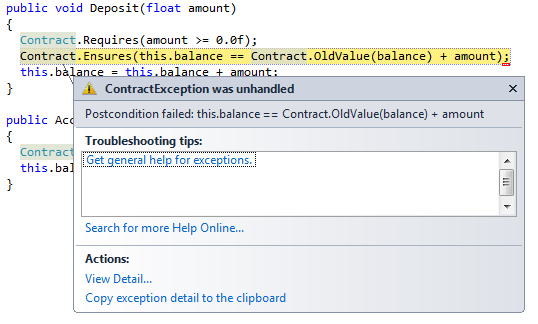
\includegraphics[width=\textwidth]{PostConditionFailed.png}
\caption{A failure at runtime of the postcondition for \code{Deposit}.}
\label{fig:failure}
\end{figure}

\noindent
What is wrong here? Let's first rule out causes that are \emph{not}
the problem:
\begin{itemize}
\item Overflow can be excluded, as floating point numbers
cannot overflow (at worst, operations result in special values $\pm \infty$ or \code{NaN}).

\item Non-determinism  is ruled out by the IEEE754 standard, and by the fact that the code in the example is single-threaded. 

\item Cancellation is to be ruled out too: \emph{e.g.} the numerical quantities are positive and of the same order of magnitude.

\item Floating point addition is commutative, so this is not the cause of the problem either. 

\item Addition is \emph{not} necessarly associative, but we do not need associativity here (we are adding only two numbers).
\end{itemize}
The real culprit here is the equality test. In general all comparisons of floating point values are problematic. 
However it is still unclear at first sight why the comparison is a
source of problems here: after all we are adding up the same two quantities and then comparing them for equality.
If some  rounding error occurs, then the same error should occur
in both additions, or won't it?

The reason for the unexpected behavior is to be found deeper in the specification of the Common Language Runtime (Partition I, Sect. 12.1.3 of \cite{CLR}):

\begin{quote}\itshape\small
Storage locations for floating-point numbers (statics, array elements, and fields of classes) are of fixed size. 
The supported storage sizes are \Float and \Double. 
Everywhere else (on the evaluation stack, as arguments, as return types, and as local variables) \textbf{floating-point numbers are represented using an internal floating-point type}. 
In each such instance, the nominal type of the variable or expression is either \Float or \Double, but its value can be represented internally with additional range and/or precision. 
The size of the internal floating-point representation is implementation-dependent, can vary, and shall have precision at least as great as that of the variable or expression being represented. An implicit widening conversion to the internal representation from \Float or \Double is performed when those types are loaded from storage.
[...]
\textbf{When a floating-point value whose internal representation has greater range and/or precision than its nominal type is put in a storage location, it is automatically coerced to the type of the storage location}.
\end{quote}

\noindent
The standard allows exploiting the maximum precision
available from the floating point hardware for operations on values in
registers \emph{despite} of their nominal type, \emph{provided} that on memory stores the internal value is truncated to the nominal size.
It is now easy to see why we get the postcondition violation at runtime.

The result of the evaluation of the expression \code{this.balance + amount} is internally stored at the maximum precision available from the hardware (on Intel processors 80 bits registers, on ARM architectures 64 bits).
In the example, the result of the addition is \code{9.42477822}, a
value that cannot be precisely represented in \code{32} bits.

The successive field store forces the value to be truncated to 32
bits, thereby changing the value.
In the example, \code{9.42477822} is coerced to a \code{float},
causing a loss of precision resulting in the value \code{9.424778} being stored in the field \code{this.balance}.

When the postcondition is evaluated,  the truncated value of \code{balance} is
re-loaded from memory, but the addition in the postcondition is re-computed with the internal precision.
Comparing these two values causes the postcondition to fail, since \code{9.424778} $\not=$ \code{9.42477822}.

\subsubsection*{Contribution}

We present a simple static analysis to check that floating point comparisons (equalities, inequalities) use operands of \emph{compatible} types.
When they are not compatible, the analysis reports a warning message to the user, so that all successive validations should be understood as conditional.
We fully implemented the analysis in Clousot, our static contract
checker based on abstract interpretation for
.NET~\cite{MafLogozzo10}. We validated the analysis by running it on
the base class library of .NET where it emitted 5 real warnings.


\begin{figure}[t]
\begin{center}
\small
\begin{tabular}{l l c l l}
  \code{l}  =  $k$                                & \textit{(load const)} & \hspace{1cm} &   \\
  \code{l}  = \code{l_1}                           & \textit{(copy)}       &              & \code{l}            =  \code{(\code{type})} \code{l_1}  & \textit{(cast)}\\
  \code{l}  =  \code{l_1} \textit{op} \code{l_2}   & \textit{(binary op)}  &            & \\     
  \code{l}  =  \code{o.f}                         & \textit{(load field)} &             & \code{o.f}            =  \code{l}                      & \textit{(store field)} \\
  \code{l}  =  \code{a[l_i]}                        & \textit{(load array)} &             & \code{a[l_i]}  =  \code{l}                      & \textit{(store array)} \\
\end{tabular}
\caption{The simplified bytecode language we consider for the analysis. A constant $k$ can only be a constant belonging to the  \Float or \Double ranges. Casting is allowed only to  $\code{type} \in \{ \Float, \Double \} $.}
\label{fig:language}
\end{center}
\end{figure}

\section{The Language}
We illustrate our analysis on a minimalistic bytecode language.
We make some simplyfing assumptions.
There are two kinds of variables: store variables ($\code{f, a} \in \code{S}$) and locals ($\code{l, p} \in \code{L}$). 
\emph{Store} variables are instance fields, static fields and arrays.
\emph{Local} variables are locals, parameters, and the return value.
Variables belong to the set $\code{Vars} = \code{S} \cup \code{L}$. 
Aliasing is not allowed.

The language has only two nominal floating point types ($\Float, \Double \in \code{T_N}$ ) and one internal floating point type (\Internal) such that $64 \leq \code{X}$.
On \code{x86}, \Internal is \code{float80}, allowing  extended floating point   precision. 
Please note that the \code{.NET} standard does not include a \code{long\ double} as for instance C~\cite{C}, so application programmers have no access to  \Internal types.

All variables have a nominal floating point type.
At runtime, the nominal floating point type for locals may be widened
but not that of store variables. We say ``may be widened'', as it
depends on register allocation choices by the compiler. We think it is
reasonable to force the code to compute values independent of floating
point register allocation choices.

The simplified bytecode language is presented in Fig.~\ref{fig:language}.
Floating point constants  are loaded into locals \textit{(load const)}.
Admissible constant values are only those admitted by the nominal types, \emph{i.e.} floating point constants in $32$ or $64$ bits including special values as $\pm \infty$ and \code{NaN} (Not-a-number).

Values can be copied to locals, retaining their internal value \textit{(copy)}.
Casting is allowed only to nominal types, with values  narrowed or widened as needed  \textit{(cast)}.
In general it is not true that if \code{l_1} and \code{l} have the same \emph{nominal} type then \textit{(cast)} is semantically equivalent to \textit{(copy)} as their \emph{internal} type may differ.

Binary operations  are the usual floating point arithmetic ones ($+, -, *, /$) and (unordered) comparison operations ($\code{==, <, \leq,}$) \textit{(binary op)}.  
The result of a comparison is $0.0$ if the comparison is false, $1.0$ otherwise.

Values are loaded from and stored to fields \textit{([load/store] field)}.
We do not distinguish between static and instance fields. 
Fields only contain values of nominal types:
therefore, when storing a local into a field, its value is automatically narrowed to the field nominal type value.
If the value of \code{l} is too large or too small, then it is approximated to $\pm \infty$ or to $0$.
Similarly, values read from arrays have a nominal type value and values written into arrays are narrowed to the nominal type of the array type.
Arrays are indexed by local values, and in addition to the usual out-of-bounds  checking, we assume that the computation stops also when \code{l_i} is a floating point number with non-zero decimal part or it is \code{NaN}.

\begin{example}
The compilation to simplified bytecode of the body of  method \code{deposit} (without contracts) of Fig.~\ref{fig:example} is in Fig.~\ref{fig:compilation}.
Please note that the store and load field operations are now made explicit in the bytecode.
\end{example}

\begin{figure}[t]
\begin{center}
\small
\begin{tabular}{l l l l}
\code{0:} & \code{l_1}           & = & \code{this.balance} \\
\code{1:} &\code{l_2}           & = & \code{amount} + \code{l_1} \\
\code{2:} &\code{this.balance}  & = & \code{l_2} \\
\code{3:} &\code{l_1}           & = & \code{this.balance} \\
\code{4:} &\code{l_{comp}}       & = & \code{l_1} \code{==} \code{l_2}
\end{tabular}
\caption{The (partial) compilation of the running example in our simple bytecode instruction set.}
\label{fig:compilation}
\end{center}
\end{figure}


\section{The Abstract Semantics}

\subsection{Abstract Domain}
The abstract domain $\mathcal{T}$ we use captures the potential
runtime floating point width a variable may have, which may be more precise than its nominal type.
Therefore, the elements of $\mathcal{T}$ belong to the set $\code{Vars} \longrightarrow \code{T_X}$ where $64 \leq \code{X}$ and  \code{T_X} is the abstract domain:

\[
\xymatrix {
       & \top &  \\
\Float \ar[ur] & \Double \ar[u] & \Internal \ar[ul] \\
       & \ar[ul] \ar[u] \ar[ur] \bottom &
}
\]

If $\code{X} = 64$, \emph{i.e.} the hardware does not provide any wider floating point register, then \Double and \Internal co-incide.
This is the case on ARM architectures, but not for \code{x86} architectures which provide extra precision registers.

The operations of the abstract domain $\mathcal{T}$ (order, join, meet) are the functional pointwise extensions of those on the lattice above.
No widening is required as the lattice is of finite height.


\begin{figure}[t]
\begin{center}
\small
\begin{tabular}{l l l}
  \sem{\code{l}   =  \mathit{k}}($\tau$)                       & = & $\tau$[\code{l} $\mapsto$ $\eta$(\code{l})]                       \\
  \sem{\code{l}   =  \code{l_1}}($\tau$)                        & = & $\tau$[\code{l} $\mapsto$ $\tau$(\code{l_1})] \\
  \sem{\code{l}   =  \code{(\code{type})} \code{l_1}}($\tau$)    & = & $\tau$[\code{l} $\mapsto$ \code{type}]\\
  \sem{\code{l}   =  \code{l_1} \textit{op} \code{l_2}}($\tau$) & = &   $\tau$[\code{l} $\mapsto$ \Internal]\\     
  \sem{\code{l}   =  \code{o.f}}($\tau$)                        & = &  $\tau$[\code{l} $\mapsto$ $\eta$(\code{o.f})]\\
  \sem{\code{o.f} =  \code{l}}($\tau$)                          & = & $\tau$ \\
  \sem{\code{l}   =  \code{a[l_i]}}($\tau$)                     & = &  $\tau$[\code{l} $\mapsto$ $\eta$(\code{a[\cdot]})\\
  \sem{\code{a[l_i]} =  \code{l}}($\tau$)                       & = & $\tau$ \\
\end{tabular}
\caption{The abstract semantics. The function $\eta$ returns the nominal type of a variable.}
\label{fig:abstractsemantics}
\end{center}
\end{figure}

\subsection{Abstract Semantics}
The abstract semantics $\sem{\cdot} \in \code{P} \times \mathcal{T} \longrightarrow \mathcal{T}$ statically determines, at each program point an internal type for each local variable.
Store variables are known, by the ECMA standard, to have their nominal type coincide with the internal type.

The abstract transfer function is defined in Fig.~\ref{fig:abstractsemantics}.
The only  constant values that can be explicitly represented are those admissible as \Float or \Double values:
the internal type of a local after a load constant is its nominal type.
Variable copy retains the internal type.
The ECMA standard guarantees that casting a value $v$ to \code{type} truncates the value $v$  to one in the \code{type} range. 
If $v$ is too large or too small for \code{type} then it is rounded to $\pm \infty$ or $0$.
The result of a binary operation is a value of maximum hardware precision, which we denote by \Internal. 
Reading from a field or an array location provides a value of the nominal type (no extra precision can be stored in fields).
Writing into a field or an array location causes the truncation of the value to the corresponding nominal type. 


\begin{example}
For the bytecode in Fig.~\ref{fig:compilation}, with $\tau_{0} = [\code{amount} \mapsto \Internal]$, the inferred internal types after each program point are:

{\small
\begin{tabular}{l l}
\code{0:} & $\tau_1 = \tau_0[\code{l_1} \mapsto \Float]$ \\
\code{1:} & $\tau_2 = \tau_1[\code{l_2} \mapsto \Internal]$\\
\code{2:} & $\tau_3 = \tau_2$\\
\code{3:} & $\tau_4 = \tau_3[\code{l_1} \mapsto \Float]$\\
\code{4:} & $\tau_5 = \tau_4[\code{l_{comp}} \mapsto \Internal]$
\end{tabular}
}
\end{example}

\subsection{Checking}

Checking a program \code{P} for precision mismatch in floating point comparisons is now quite easy.
First run the analysis \sem{P} to collect an over-approximation of the
internal types for each program point.
Then, for each \textit{(binary op)} in \code{P}
\[
\code{pp}:  \code{l}  =  \code{l_1} \mathop{\textit{op}}\, \code{l_2}  
\]
such that  \textit{op} is one of \code{==, \leq, <} get $\tau_{pp}$, which is the abstract pre-state for \code{pp}. 

If $\tau_{pp}(\code{l_1})$ or $\tau_{pp}(\code{l_2})$ are different from $\top$, and $\tau_{pp}(\code{l_1}) = \tau_{pp}(\code{l_2})$ then the comparison is on variables with the same internal type.
Otherwise, the comparison may happen on floating point values of different width, and hence a warning to the user should be emitted.

\begin{example}
In our running example, $\tau_5(\code{l_{2}}) = \Internal$ and  $\tau_5(\code{l_{1}}) = \Float$.
So a warning is emitted to the user (cf. Fig~\ref{fig:warning}).
\end{example}

\begin{figure}[t]
  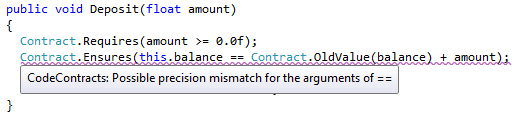
\includegraphics[width=\textwidth]{ClousotMessage.png}
\vspace*{-10mm}
\caption{The warning emitted by Clousot.}
\label{fig:warning}
\end{figure}

\subsection{Fixing the warnings}

When the analysis cannot prove that the operands of a comparison are of the same type, the user can fix it by adding explicit casts.
For instance in our running example, the right postcondition is one
where the type coercion is made explicit:
\begin{lstlisting}
  Contract.Ensures(balance == (float)Contract.OldValue(balance) + amount);
\end{lstlisting}
From a programmer's point of view, this coercion seems redundant, as
the expression \code{Contract.OldValue(balance) + amount} already has
nominal type \Float. He/she may expect that the explicit cast to
\Float would be a  no-operation. But for the reasons explained in this
paper, the cast may be a truncation.


\section{Implementation and Experiment}

We have implemeted the  analysis described in this paper in Clousot, our static analyzer for CodeContracts~\cite{MafLogozzo10}.
The analyzer first reads the IL from disk, then constructs for each
method the control flow graph, inserting  contracts at the necessary points.
Then it simplifies the program by getting rid of the evaluation stack
and the heap, reconstructs expressions lost during compilation, and
finally produces a \emph{scalar} program.

Several analyses are run on the top of the scalar program, \emph{i.e.}
non-null, numerical, array, or arithmetic. We added the detection of precision
mismatches in floating point
comparisons described in this paper to the arithmetic analysis.
The
analysis is fast and accurate: on the core library of the \code{.NET}
framework, \code{mscorlib.dll}, constisting of 25089 methods, it
adds less than 10 seconds to the total time, and it reports 5 warnings.  We manually inspected those, and they all
represent real warnings similar to the following example:
\begin{lstlisting}
  bool IsNonZero(float f) {
    return f != 0.0F;
  }
\end{lstlisting}
According to the ECMA standard, the parameter \code{f} of callers may
be passed in registers and thus use more bits than \Float in
memory. Therefore, the inequality comparison against \code{0.0F} may result in \code{true}, even
though \code{f} truncated to \Float is equal to \code{0.0F}. As an
example of where this could result in problems, consider:
\begin{lstlisting}
  class C {
    float a; // should never be 0.0F

    void Update(float f) {
      if (IsNonZero(f)) {
        this.a = f;
      }

    ...
\end{lstlisting}
In the above code, the programmer expects to guard the assignment to
the field to make sure the value stored in the field is never
\code{0.0F}. However, due to register allocation of \code{f}, a value
represented using more than 32 bits, close to \code{0.0F} but not
equal to \code{0.0F} can pass the test and be truncated to \code{0.0F}
when stored into \code{this.a}.

\section{Discussion}
\label{sec:discussion}
Some languages and compilers have addressed the problem described in
this paper using other means. C compilers  typically offer
compile-time switches to control whether the compiler should emit code
that adheres strictly to the bit-widths declared in types, or whether
it is allowed to use extra precision for computations in registers.

Using strict adherence to the declared types requires compilers to
emit truncating casts after each floating point operation that could
result in more precision, or putting the floating point unit into a
mode that automatically performs truncation~\cite{Monniaux08}. 
The Java standard provides the \code{strictfp} keyword to enforce this truncating behavior and thereby avoids the problem
described in this paper entirely at the cost of precision and speed.

We decided to detect problems with precision mismatches only when
comparing floating point numbers. Another view would be to write an
analysis that warns users whenever some higher precision float is
implicitly cast to the nominal type width (effectively whenever a
result is stored into memory). The problem with such an alternative
analysis is that it would a) warn about most memory writes, b) miss
implicit narrowings arising due to register spilling into memory
introduced by the compiler. We found that warning about comparisons
addresses the problem in a more actionable way.

\section{Related Work}
Previous work in this area focuses on enhancing static analysis
techniques to soundly analyze programs with floating points.  For
instance \cite{GoubaultPutot11,Martel02,Martel02b} present static
analyses to spot the source of imprecision in floating point
computations. \cite{Mine04} introduces ideas to extend numerical
abstract domains to the analysis of IEEE 754-compliant floating point
values and \cite{Martel09} introduces program transformation
techniques to reduce the error in floating point computations.

Our work is orthogonal to those in that we are not interested in the
actual \emph{values} of the computation but only in detecting
situations that may cause unexpected comparison results. The need for
such detection is particularly important to avoid runtime failures of
contracts that seemingly have been validated via symbolic execution.

\section{Conclusions}
We described a simple static analysis to detect the absence of
``surprising'' behaviors of comparisons involving floating point
numbers.  The analysis is motivated by feeedback from users of our
Code Contract tools. They reported false negatives similar to the example
described in the introduction.  We integrated the analysis in the
static checker tool for Code Contracts, and experience shows it to be accurate enough.


\emph{Thanks.} Many thanks to Matthias Jauernig, who was the first to
report the unsoundess in Clousot illustrated here. Thanks also to Juan
Chen for the detailed explanation of the floating point subsystem in
the ARM architecture.

\bibliographystyle{plain}
\bibliography{bib}

\end{document}
